\documentclass[aspectratio=169,11pt]{beamer}
\usetheme[progressbar=frametitle,numbering=fraction]{metropolis}
\usepackage{amsmath,amssymb}
\usepackage{booktabs}
\usepackage{siunitx}
\usepackage{tikz}
\usetikzlibrary{positioning,arrows.meta,fit,backgrounds}

\graphicspath{{../report/figures/}}
\newcommand{\Q}{\mathcal{Q}}

\title{Binary Data and Spread-Spectrum Communications}
\subtitle{42057 Space Communications and Sensing --- Assignment 2, Topic 2}
\author{Benjamin Hudson [24742900], Elina Kim [24949885], \\ Rhyse Williams [24817532], Jaylen Avtarovski [24767939]}
\date{Spring 2026}

\begin{document}

\maketitle

% ----------------------------------------------------------------
\begin{frame}{Why spread spectrum in space links? - Benjamin}
\begin{itemize}
  \item Space links are power limited and exposed to interference and jamming.
  \item GPS spreads a \SI{50}{bit/s} message with a \SI{1.023}{Mchips/s} code:
        \alert{\SI{43}{dB} processing gain}.
  \item PN DSSS allows for discrete transmission with intrinsic time codeing
\end{itemize}
\vspace{0.4cm}
\textbf{Our task}
\begin{enumerate}
  \item Simulate a binary system in uniform noise and measure BER vs SNR.
  \item Add a PN sequence and a sinusoidal jammer $A\sin\omega_0 n$, $A\ge M$,
        and compare with and without PN for $M=50,100,500,1000$.
\end{enumerate}
\end{frame}

% ----------------------------------------------------------------
\begin{frame}{System models - Benjamin}
\centering
\resizebox{0.95\textwidth}{!}{%
\begin{tikzpicture}[
  blk/.style={draw, rounded corners=2pt, minimum height=0.8cm, minimum width=1.5cm,
              align=center, font=\scriptsize, fill=mLightBrown!15},
  op/.style={draw, circle, inner sep=0pt, minimum size=0.45cm, font=\scriptsize},
  >={Stealth[length=2mm]}, node distance=0.4cm]
  \node[blk] (src) {Binary\\data};
  \node[blk, right=of src] (mod) {Modulator\\$\pm1\times M$};
  \node[op, right=0.5cm of mod] (x1) {$\times$};
  \node[op, right=0.7cm of x1] (a1) {$+$};
  \node[op, right=1.1cm of a1] (a2) {$+$};
  \node[op, right=1.5cm of a2] (x2) {$\times$};
  \node[blk, right=0.5cm of x2] (dem) {Demod.\\$\sum_M$};
  \node[blk, right=of dem] (det) {Detector\\$y_k\gtrless0$};
  \node[blk, below=0.4cm of x1, fill=mLightGreen!25] (pn1) {PN $p(n)$};
  \node[blk, above=0.4cm of a1, fill=red!12] (sin) {$A\sin\omega_0 n$};
  \node[blk, below=0.4cm of a2] (noi) {$w(n)\sim\mathcal{U}(-a,a)$};
  \node[blk, below=0.4cm of x2, fill=mLightGreen!25] (pn2) {PN $p(n)$};
  \draw[->] (src) -- (mod); \draw[->] (mod) -- node[above,font=\tiny]{$s(n)$} (x1);
  \draw[->] (x1) -- (a1); \draw[->] (a1) -- (a2); \draw[->] (a2) -- (x2);
  \draw[->] (x2) -- (dem); \draw[->] (dem) -- (det);
  \draw[->] (pn1) -- (x1); \draw[->] (sin) -- (a1); \draw[->] (noi) -- (a2); \draw[->] (pn2) -- (x2);
\end{tikzpicture}}

\vspace{0.4cm}
\begin{columns}[T]
\column{0.48\textwidth}
\textbf{Project 12.7}: green and red blocks removed.\\
$y_k = \pm M + \sum w(n)$, \quad $\mathrm{SNR}=M/P_n$, \quad $P_n=a^2/3$.
\column{0.48\textwidth}
\textbf{Project 12.8}: full diagram.\\
Same PN at both ends, $p^2(n)=1$, so the signal is restored exactly.
\end{columns}
\end{frame}

% ----------------------------------------------------------------
\begin{frame}[fragile]{MATLAB implementation - Benjamin}
\begin{columns}[T]
\column{0.5\textwidth}
One function per block, reused across both projects:
\begin{itemize}\small
  \item \texttt{bit\_generator}, \texttt{modulator}
  \item \texttt{noise\_generator}, \texttt{demodulator}
  \item \texttt{detector} (and error counter)
  \item \texttt{pn\_generator}, \texttt{sine\_generator}
  \item \texttt{binary\_comm\_sim}: Monte-Carlo loop
\end{itemize}
\small No toolboxes; block-wise processing for $M=1000$;\\
run until 200 errors or $2\times10^7$ bits.
\column{0.5\textwidth}
\begin{block}{Core loop}
\scriptsize
\begin{verbatim}
b = bit_generator(Nb);
s = modulator(b, M);
if use_pn, p = pn_generator(L); s = s.*p; end
r = s + noise_generator(L, a) ...
      + sine_generator(L, A, w0, n0);
if use_pn, r = r.*p; end
y = demodulator(r, M);
[~, e] = detector(y, b);
\end{verbatim}
\end{block}
\end{columns}
\end{frame}

% ----------------------------------------------------------------
\begin{frame}{Project 12.7: signals through the system - Elina}
\centering
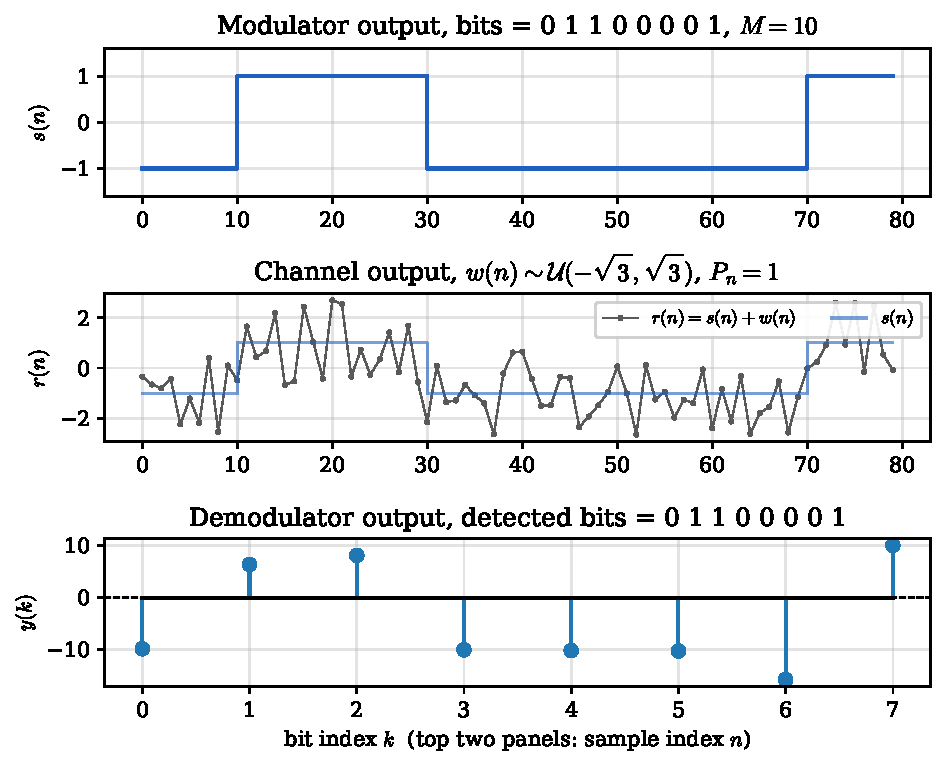
\includegraphics[height=0.8\textheight]{p127_waveforms}
\end{frame}

% ----------------------------------------------------------------
\begin{frame}{Project 12.7: BER vs SNR - Elina}
\begin{columns}[c]
\column{0.58\textwidth}
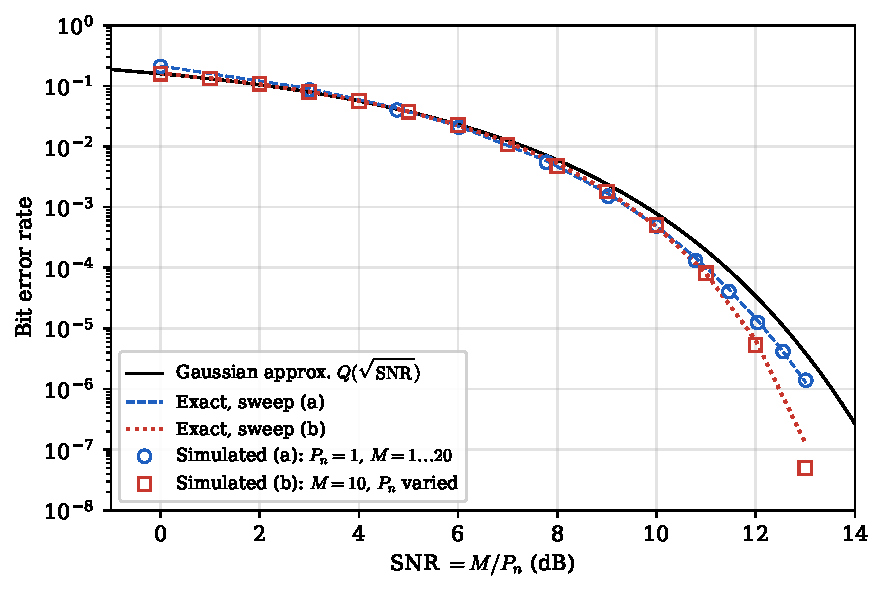
\includegraphics[width=\linewidth]{p127_ber}
\column{0.42\textwidth}
\small
\begin{itemize}
  \item Exact closed-form (Irwin--Hall) result lies inside the \alert{95\% interval}
        at 25 of 26 points, as expected; the lowest BERs rest on few errors.
  \item $\Q(\sqrt{\mathrm{SNR}})$ is \alert{pessimistic} at high SNR: uniform noise is bounded.
  \item Sweeps diverge at high SNR: with $M=10$ fixed, $a\to1$ and errors become
        impossible ($Ma\le M$).
\end{itemize}
\end{columns}
\end{frame}

% ----------------------------------------------------------------
\begin{frame}{Theory: what the PN sequence does to the jammer - Elina}
\begin{columns}[T]
\column{0.5\textwidth}
\textbf{Without PN}
\[
  J_k = A\,\frac{\sin(M\omega_0/2)}{\sin(\omega_0/2)}\sin(\cdot)
\]
\small
\begin{itemize}
  \item In-band ($\omega_0\ll2\pi/M$): $|J_k|\to AM$, integrated like the signal.
  \item Out-of-band: $|J_k|\le A/\sin(\omega_0/2)$, already filtered.
\end{itemize}
\column{0.5\textwidth}
\textbf{With PN}
\[
  \mathrm{Var}[J_k'] \approx \frac{MA^2}{2},\quad
  P_e\approx\Q\!\left(\sqrt{\frac{M}{P_n + A^2/2}}\right)
\]
\small
\begin{itemize}
  \item Jammer becomes white noise of power $A^2/2$.
  \item Processing gain $G_p = M$ (\SIrange{17}{30}{dB}).
  \item But $A=M$ means $\mathrm{JSR}=M^2/2$: \alert{SINR $\approx 2/M$}.
\end{itemize}
\end{columns}
\end{frame}

% ----------------------------------------------------------------
\begin{frame}{Project 12.8: spectra before and after despreading - Rhyse}
\begin{columns}[c]
\column{0.58\textwidth}
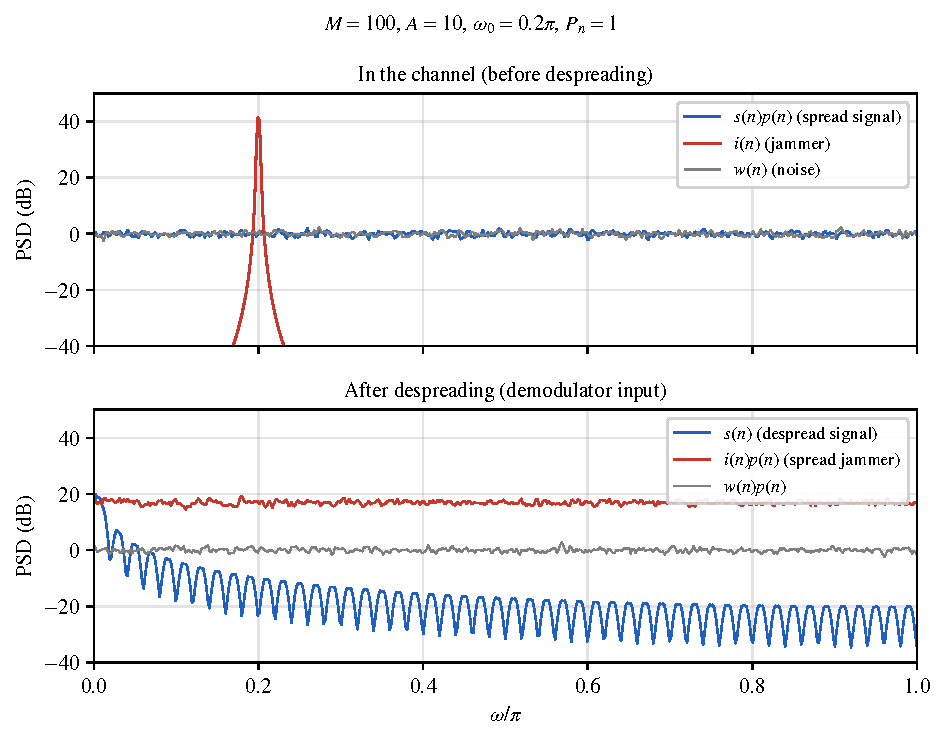
\includegraphics[width=\linewidth]{p128_spectra}
\column{0.42\textwidth}
\small
$M=100$, $A=10$, $\omega_0=0.2\pi$
\begin{itemize}
  \item Channel: signal is white at \SI{0}{dB}, jammer is a \SI{40}{dB} line.
  \item After despreading: signal returns to a $\mathrm{sinc}^2$ with \SI{20}{dB}
        at DC; jammer is a \alert{white floor} at \SI{17}{dB}.
  \item The demodulator is a \alert{low-pass} response: its main lobe ($|\omega|<2\pi/M$) holds most of the signal energy but only about $1/M$ of the jammer power.
\end{itemize}
\end{columns}
\end{frame}

% ----------------------------------------------------------------
\begin{frame}{Project 12.8: the brief's experiment, $A=M$ - Rhyse}
\begin{columns}[c]
\column{0.58\textwidth}
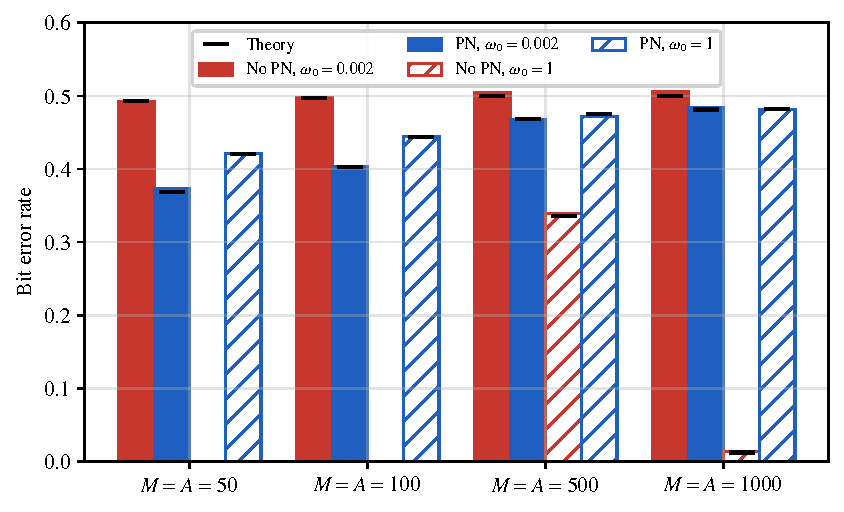
\includegraphics[width=\linewidth]{p128_ber_A_eq_M}
\column{0.42\textwidth}
\small
\begin{itemize}
  \item \textbf{In-band}: no PN $\approx0.5$; PN $0.37$ at $M=50$, rising to $0.48$.
  \item \textbf{Out-of-band}: no PN is often \emph{better}; the integrator rejects the tone.
  \item Theory (black ticks) matches within $0.007$.
  \item JSR of \SIrange{31}{57}{dB} exceeds the processing gain.
\end{itemize}
\end{columns}
\end{frame}

% ----------------------------------------------------------------
\begin{frame}{Processing gain: BER vs jammer power - Rhyse}
\begin{columns}[c]
\column{0.58\textwidth}
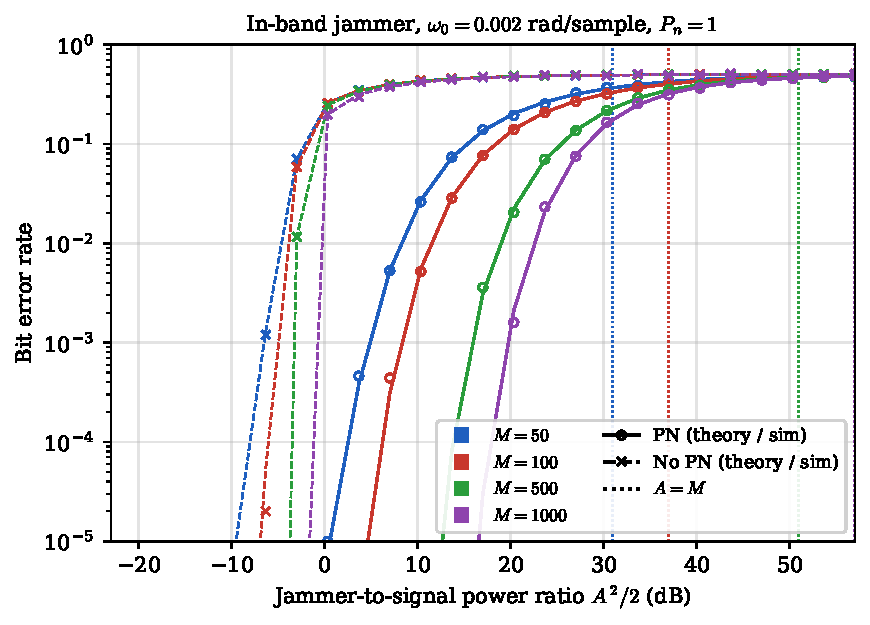
\includegraphics[width=\linewidth]{p128_ber_vs_jsr}
\column{0.42\textwidth}
\small
JSR tolerated at BER $=10^{-3}$:
\begin{center}
\begin{tabular}{@{}rccc@{}}
\toprule
$M$ & No PN & PN & Improvement \\
\midrule
50   & $-6.5$ & $4.9$  & \SI{11.4}{dB} \\
100  & $-5.0$ & $8.3$  & \SI{13.3}{dB} \\
500  & $-3.3$ & $16.0$ & \SI{19.2}{dB} \\
1000 & $-0.7$ & $19.7$ & \SI{20.5}{dB} \\
\bottomrule
\end{tabular}
\end{center}
Without PN, more samples per bit \alert{do not help}: the jammer is integrated too.
\end{columns}
\end{frame}

% ----------------------------------------------------------------
\begin{frame}{BER vs jammer frequency ($M=100$) - Jaylen}
\begin{columns}[c]
\column{0.55\textwidth}
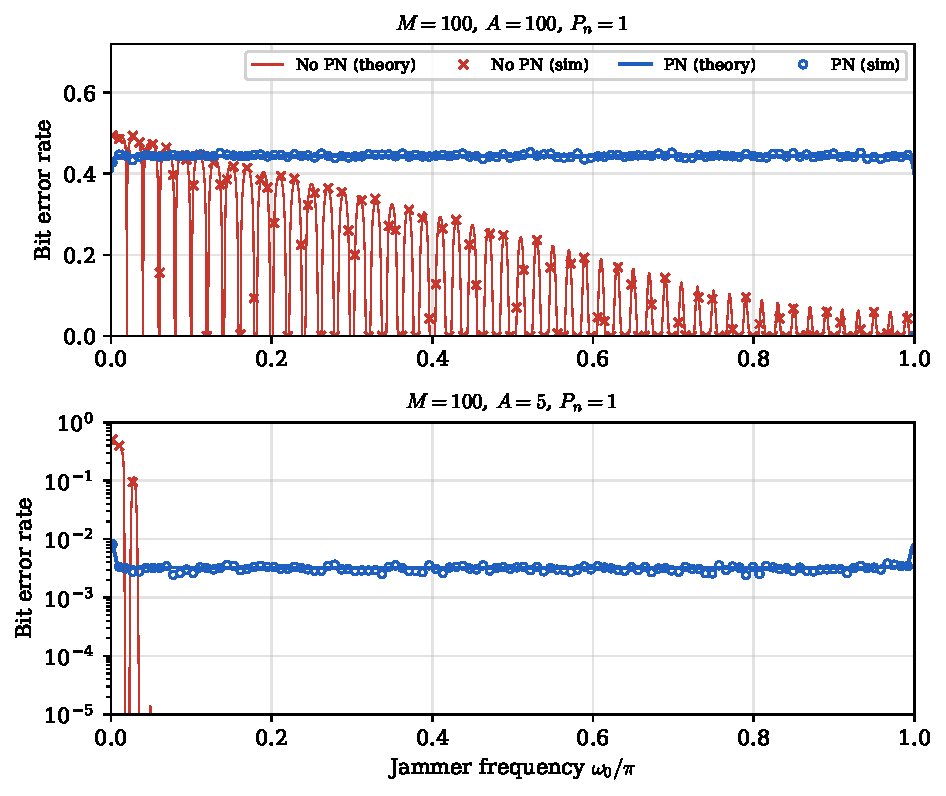
\includegraphics[width=\linewidth]{p128_ber_vs_w0}
\column{0.45\textwidth}
\small
\begin{itemize}
  \item PN: BER is \alert{nearly flat in frequency}; it changes only within $\sim2\pi/M$
        of $0$ and $\pi$.
  \item No PN: BER follows the Dirichlet kernel, zero at the nulls $2\pi\ell/M$,
        worst near $\omega = 0$.
  \item A jammer can always pick the conventional receiver's weak spot: the signal band.
\end{itemize}
\end{columns}
\end{frame}

% ----------------------------------------------------------------
\begin{frame}{Why spread spectrum wins (and when it doesn't) - Jaylen}
\begin{enumerate}
  \item \textbf{Coherent vs incoherent addition}: the signal sums to $M$ (power $M^2$),
        the despread jammer to power $MA^2/2$, a gain of $M$.
  \item \textbf{Weak frequency dependence}: away from the band edges there is no weak frequency to exploit.
  \item \textbf{Low probability of intercept and CDMA}: the signal sits at the noise floor.
\end{enumerate}
\vspace{0.3cm}
\begin{alertblock}{Caveat from the $A\ge M$ condition within the brief}
Jammer power grows as $M^2$ but processing gain only as $M$, so PN sits near BER $=0.5$.
No PN: also $\approx0.5$ in band, but an out-of-band tone is filtered out (BER $0$--$0.013$, except $0.33$ at $M=500$).
\end{alertblock}
\end{frame}

% ----------------------------------------------------------------
\begin{frame}{Conclusions - Jaylen}
\begin{itemize}
  \item Modular MATLAB simulator, one function per block, validated against exact theory.
  \item 12.7: BER matches the exact uniform-noise result; the Gaussian
        approximation is pessimistic at high SNR.
  \item 12.8: PN de-spreading turns a tone into white noise, giving
        \SIrange{11.4}{20.5}{dB} measured improvement (ideal \SIrange{17}{30}{dB}) for $M=50$ to $1000$ and
        nearly frequency-independent performance.
  \item With $A=M$ the jammer exceeds the ideal processing gain by \SIrange{14}{27}{dB}; the outcome then depends on jammer frequency.
  \item Limitations: perfect synchronisation; random PN instead of m-sequences or Gold codes.
\end{itemize}
\end{frame}

\begin{frame}[standout]
Questions?
\end{frame}

\end{document}
